\documentclass[../physics12.tex]{subfiles}
\graphicspath{{\subfix{../figures/}}}
\begin{document}
\chapter{Induction and AC Circuits}
\section{Formulas}
Faraday's law of induction: $\Delta V = -N\Delta \varphi_B/\Delta t$ where the magnetic flux $\varphi_B = BA\cos\theta$

Induced emf in a wire moving $\perp$ to a magnetic field (Hall Effect): $\Delta V = \epsilon = Blv$

Induced emf in a wire moving in a magnetic field: $\Delta V = Blv\sin\theta$

Maximum emf in a generator: $\Delta V = NBA\omega$

Definition of self inductance $L$: $\Delta V = -L\Delta I/\Delta t$

Energy stored in an inductor: $U = LI^2/2$

RL circuit with $I_0 = 0$: $I(t) = I_{\text{max}}(1-e^{-Rt/L})$

AC current RMS value: $I_{\text{rms}} = I_{\text{max}}/\sqrt{2}$

AC voltage RMS value: $\Delta V_{\text{rms}} = \Delta V_{\text{max}}/\sqrt{2}$

Reactance of a capacitor: $X_C = \frac{1}{\omega C}=\frac{1}{2\pi f C}$

Reactance of an inductor: $X_L = \omega L = 2\pi f L$

Impedance of a series RLC circuit: $Z = \sqrt{R^2+(X_L-X_C)^2}$

Amplitudes: $V_R = IR, VL = IX_L, V_C = IX_C$, and $\epsilon = IZ$

Angular frequency at resonance: $\omega_0 = 2\pi f = \frac{1}{\sqrt{LC}}$

AC transformer: $I_1/I_2 = \Delta V_2/\Delta V_1 = N_2/N_1$

\section{Dropped Steel Beam Problem}
A 11.5 m long steel beam is accidentally dropped by a construction crane from a height of 5.41 m. The horizontal component of the Earth's 
magnetic field over the region is 12.9 $\mu$T. The acceleration of gravity is 9.8 m/s$^2$.

What is the induced emf in the beam just before impact with the Earth, assuming its long dimension remains in a horizontal plane, oriented perpendicularly to the horizontal component of the Earth's magnetic field? Answer in units of mV.

\section{Energy Stored in Inductor Problem}
An inductor of 140 turns has a radius of 5 cm and a length of 28 cm. The permeability of free space is $1.25664\times 10^{-6}$ N/A$^2$. 

Find the energy stored in it when the current is 0.4 A. Answer in units of J.

\section{Force on a Bar Problem}
In the arrangement shown in the figure, the resistor is $1 \Omega$ and a 9 T magnetic field is directed into the paper. The separation 
between the rails is 4 m. An applied force moves the bar to the right at a constant speed of 2 m/s.
\begin{center}
    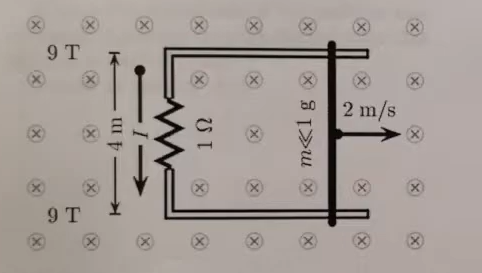
\includegraphics[width=0.5\textwidth]{12.1.PNG}
\end{center}
Calculate the applied force required to move the bar to the right at a constant speed of 2 m/s. Assume the bar and rails have negligible resistance and friction.
Neglect the mass of the bar. Answer in units of N.

\section{Rate of Change of Current in Inductor Problem}
An inductor in the form of an air-core solenoid contains 183 turns, is of length 22.7 cm, and has a cross-sectional area of 1.2 cm$^2$. The permeability of free space is $1.25664\times 10^{-6}$ N/A$^2$.

What is the magnitude of the uniform rate of change in current through the inductor that induces an emf of 275 $\mu$V? Answer in units of A/s.

\section{Change in Field of Rectangular Coil Problem}
The plane of a rectangular coil, 6.9 cm by 3.6 cm, is perpendicular to the direction of a uniform magnetic field $B$.

If the coil has 75 turns and a total resistance of $8.9 \Omega$, at what rate must the magnitude of $B$ change to induce a current of 0.04 A in the windings of the coil? Answer in units of T/s.

\section{Inductor with Series in Lamp Problem}
A 0.834 H inductor is connected in series with a fluorescent lamp to limit the current drawn by the lamp.

If the combination is connected to a 67 Hz, 125 V line, and if the voltage across the lamp is to be 46.2 V, what is the current in the circuit? (The lamp is a pure resistive load.) Answer in units of A.

\end{document}